\documentclass[tikz,border=7pt]{standalone}
\usepackage{amsmath,amssymb}
\usetikzlibrary{arrows.meta,calc,positioning,fit,decorations.pathreplacing}

\definecolor{ink}{HTML}{243447}
\definecolor{muted}{HTML}{64748B}
\definecolor{flow}{HTML}{2563A6}
\definecolor{flowLight}{HTML}{DBEAFE}
\definecolor{grad}{HTML}{C43D3D}
\definecolor{gradLight}{HTML}{FAD4D4}
\definecolor{good}{HTML}{2F855A}
\definecolor{panelFill}{HTML}{F8FAFC}

\tikzset{
    >={Latex[length=2.2mm,width=1.6mm]},
    panel/.style={draw=ink!25, fill=panelFill, rounded corners=3pt, line width=0.7pt},
    state/.style={circle, draw=ink, fill=white, line width=0.8pt,
                  minimum size=7.5mm, inner sep=0pt, font=\sffamily\scriptsize},
    mapblock/.style={rounded corners=3pt, draw=flow, fill=flowLight,
                    line width=1pt, minimum width=20mm, minimum height=25mm,
                    align=center, font=\sffamily\scriptsize},
    constraint/.style={rounded corners=3pt, draw=grad, fill=gradLight,
                      line width=1pt, minimum width=31mm, minimum height=11mm,
                      align=center, font=\sffamily\scriptsize},
    forward/.style={flow, line width=1.5pt, -{Latex[length=2.3mm]}},
    dependency/.style={ink!55, line width=0.9pt, -{Latex[length=1.8mm]}},
    backward/.style={grad, dashed, line width=1.45pt, -{Latex[length=2.2mm]}},
    title/.style={font=\sffamily\bfseries\small, text=ink},
    label text/.style={font=\sffamily\scriptsize, text=ink, align=center},
    small note/.style={font=\sffamily\tiny, text=muted, align=center},
}

\begin{document}
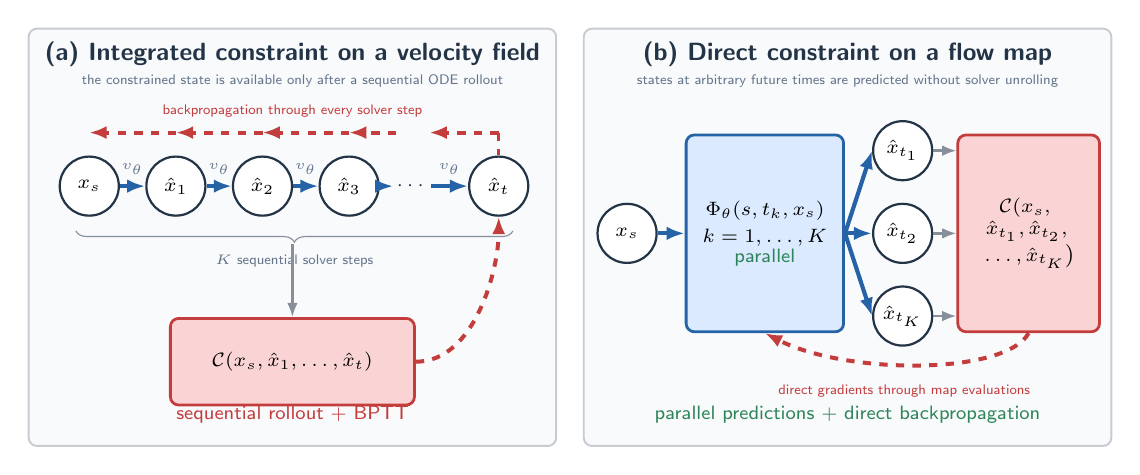
\begin{tikzpicture}[font=\sffamily]

% ---------------------------------------------------------------------------
% Panel A: velocity field
% ---------------------------------------------------------------------------
\begin{scope}[shift={(0,0)}]
    \draw[panel] (-0.25,-2.55) rectangle (6.45,2.75);
    \node[title] at (3.10,2.42) {(a) Integrated constraint on a velocity field};
    \node[small note] at (3.10,2.09)
        {the constrained state is available only after a sequential ODE rollout};

    \node[state] (x0) at (0.52,0.75) {$x_s$};
    \node[state] (x1) at (1.62,0.75) {$\hat x_1$};
    \node[state] (x2) at (2.72,0.75) {$\hat x_2$};
    \node[state] (x3) at (3.82,0.75) {$\hat x_3$};
    \node[label text] at (4.62,0.75) {$\cdots$};
    \node[state] (xk) at (5.72,0.75) {$\hat x_t$};

    \draw[forward] (x0) -- node[small note, above] {$v_\theta$} (x1);
    \draw[forward] (x1) -- node[small note, above] {$v_\theta$} (x2);
    \draw[forward] (x2) -- node[small note, above] {$v_\theta$} (x3);
    \draw[forward] (x3) -- (4.38,0.75);
    \draw[forward] (4.86,0.75) -- node[small note, above] {$v_\theta$} (xk);

    \draw[decorate, decoration={brace, amplitude=4pt, mirror}, ink!55]
        (0.35,0.18) -- (5.90,0.18)
        node[midway, below=5pt, small note] {$K$ sequential solver steps};

    \node[constraint] (costA) at (3.10,-1.48)
        {$\mathcal C(x_s,\hat x_1,\ldots,\hat x_t)$};
    \draw[dependency] (3.10,0.02) -- (costA.north);
    \draw[backward]
        (costA.east) .. controls (5.42,-1.48) and (5.72,-0.30) .. (xk.south);

    % Back-propagation path
    \draw[backward] (5.72,1.43) -- (4.84,1.43);
    \draw[backward] (4.42,1.43) -- (3.82,1.43);
    \draw[backward] (3.82,1.43) -- (2.72,1.43);
    \draw[backward] (2.72,1.43) -- (1.62,1.43);
    \draw[backward] (1.62,1.43) -- (0.52,1.43);
    \draw[grad, dashed, line width=1pt] (5.72,1.43) -- (xk.north);
    \node[small note, text=grad] at (3.10,1.70)
        {backpropagation through every solver step};
    \node[label text, text=grad] at (3.10,-2.15)
        {sequential rollout + BPTT};
\end{scope}

% ---------------------------------------------------------------------------
% Panel B: flow map
% ---------------------------------------------------------------------------
\begin{scope}[shift={(7.05,0)}]
    \draw[panel] (-0.25,-2.55) rectangle (6.45,2.75);
    \node[title] at (3.10,2.42) {(b) Direct constraint on a flow map};
    \node[small note] at (3.10,2.09)
        {states at arbitrary future times are predicted without solver unrolling};

    \node[state] (xs) at (0.30,0.15) {$x_s$};
    \node[mapblock] (map) at (2.05,0.15)
        {$\Phi_\theta(s,t_k,x_s)$\\[2pt]
         $k=1,\ldots,K$\\[-1pt]
         \textcolor{good}{\scriptsize parallel}};
    \draw[forward] (xs.east) -- (map.west);

    \node[state] (z1) at (3.80,1.20) {$\hat x_{t_1}$};
    \node[state] (z2) at (3.80,0.15) {$\hat x_{t_2}$};
    \node[state] (zk) at (3.80,-0.90) {$\hat x_{t_K}$};
    \draw[forward] (map.east) -- (z1.west);
    \draw[forward] (map.east) -- (z2.west);
    \draw[forward] (map.east) -- (zk.west);

    \node[constraint, minimum width=18mm, minimum height=25mm] (costB)
        at (5.40,0.15)
        {$\mathcal C\!\left(x_s,\right.$\\
         $\left.\hat x_{t_1},\hat x_{t_2},\right.$\\
         $\left.\ldots,\hat x_{t_K}\right)$};
    \draw[dependency] (z1.east) -- (costB.west |- z1);
    \draw[dependency] (z2.east) -- (costB.west |- z2);
    \draw[dependency] (zk.east) -- (costB.west |- zk);

    \draw[backward]
        (costB.south) .. controls (5.10,-1.65) and (3.10,-1.65) .. (map.south);
    \node[small note, text=grad] at (3.82,-1.85)
        {direct gradients through map evaluations};
    \node[label text, text=good] at (3.10,-2.15)
        {parallel predictions + direct backpropagation};
\end{scope}

\end{tikzpicture}
\end{document}
